\section{Conclusion}
\label{sec:conclusion}

In conclusion, for this second laboratory assignment, both a theoretical analysis and simulations have been presented. \par
By plotting and compiling the data obtained in tables, it is found that the simulations coincide with the theoretical predictions up until the last digit, where only some rounding errors may be found. This is due to the fact that a simple circuit is being analysed, consisted only of linear components, therefore, no approximation was required do solve the circuit. However, when analyzing more complex circuits, such as those including transistors, NGSpice may prove to be much more exact and precise. \par
In order to clearly compare the simulations from NGSpice with the theoretical predictions from octave, the tables containing the same information and the plots regarding the same events are shown side by side, where it can be seen that the results are extremely similar.


\vspace{1cm}
\begin{figure}[H]
    \minipage{0.50\textwidth}
      \centering
      \begin{tabular}{ | c | c | }
      \hline    
      {\bf Name} & {\bf Value [A or V]} \\ \hline
      \input{nodal_tab}
      \hline
      \end{tabular}
      \caption{Theoretical Question 1}
    \endminipage\hfill
    \minipage{0.50\textwidth}
      \centering
      \begin{tabular}{ | c | c | }
      \hline    
      {\bf Name} & {\bf Value [A or V]} \\ \hline
      @gb[i] & -2.24128e-04\\ \hline
@id[current] & (  )\\ \hline
@r1[i] & -2.14309e-04\\ \hline
@r2[i] & -2.24128e-04\\ \hline
@r3[i] & -9.81934e-06\\ \hline
@r4[i] & 1.183454e-03\\ \hline
@r5[i] & 1.248524e-03\\ \hline
@r6[i] & -9.69145e-04\\ \hline
@r7[i] & -9.69145e-04\\ \hline
n0 & 4.894946e+00\\ \hline
n1 & -2.98689e+00\\ \hline
n2 & 8.700499e+00\\ \hline
n3 & 4.397911e+00\\ \hline
n4 & 4.864258e+00\\ \hline
n5 & 5.082120e+00\\ \hline
n7 & -2.00234e+00\\ \hline
n8 & -2.00234e+00\\ \hline

      \end{tabular}
      \caption{Simulation Question 1}
    \endminipage\hfill
\end{figure}
\newpage
\vspace{0.1cm}
\begin{figure}[H]
    \minipage{0.50\textwidth}
      \centering
      \begin{tabular}{ | c | c | }
      \hline    
      {\bf Name} & {\bf Value [A or V]} \\ \hline
      \input{req_tab}
      \hline
      \end{tabular}
      \caption{Theoretical Question 2}
    \endminipage\hfill
    \minipage{0.50\textwidth}
      \centering
      \begin{tabular}{ | c | c | }
      \hline    
      {\bf Name} & {\bf Value [A or V]} \\ \hline
      \input{opeq_tab}
      \end{tabular}
      \caption{Simulation Question 2}
    \endminipage\hfill
\end{figure}
\vspace{0.1cm}
\begin{figure}[H]
    \minipage{0.5\textwidth}
      \includegraphics[width=\linewidth]{natural_tab.pdf}
      \caption{Theoretical Question 3}
    \endminipage\hfill
    \minipage{0.5\textwidth} 
      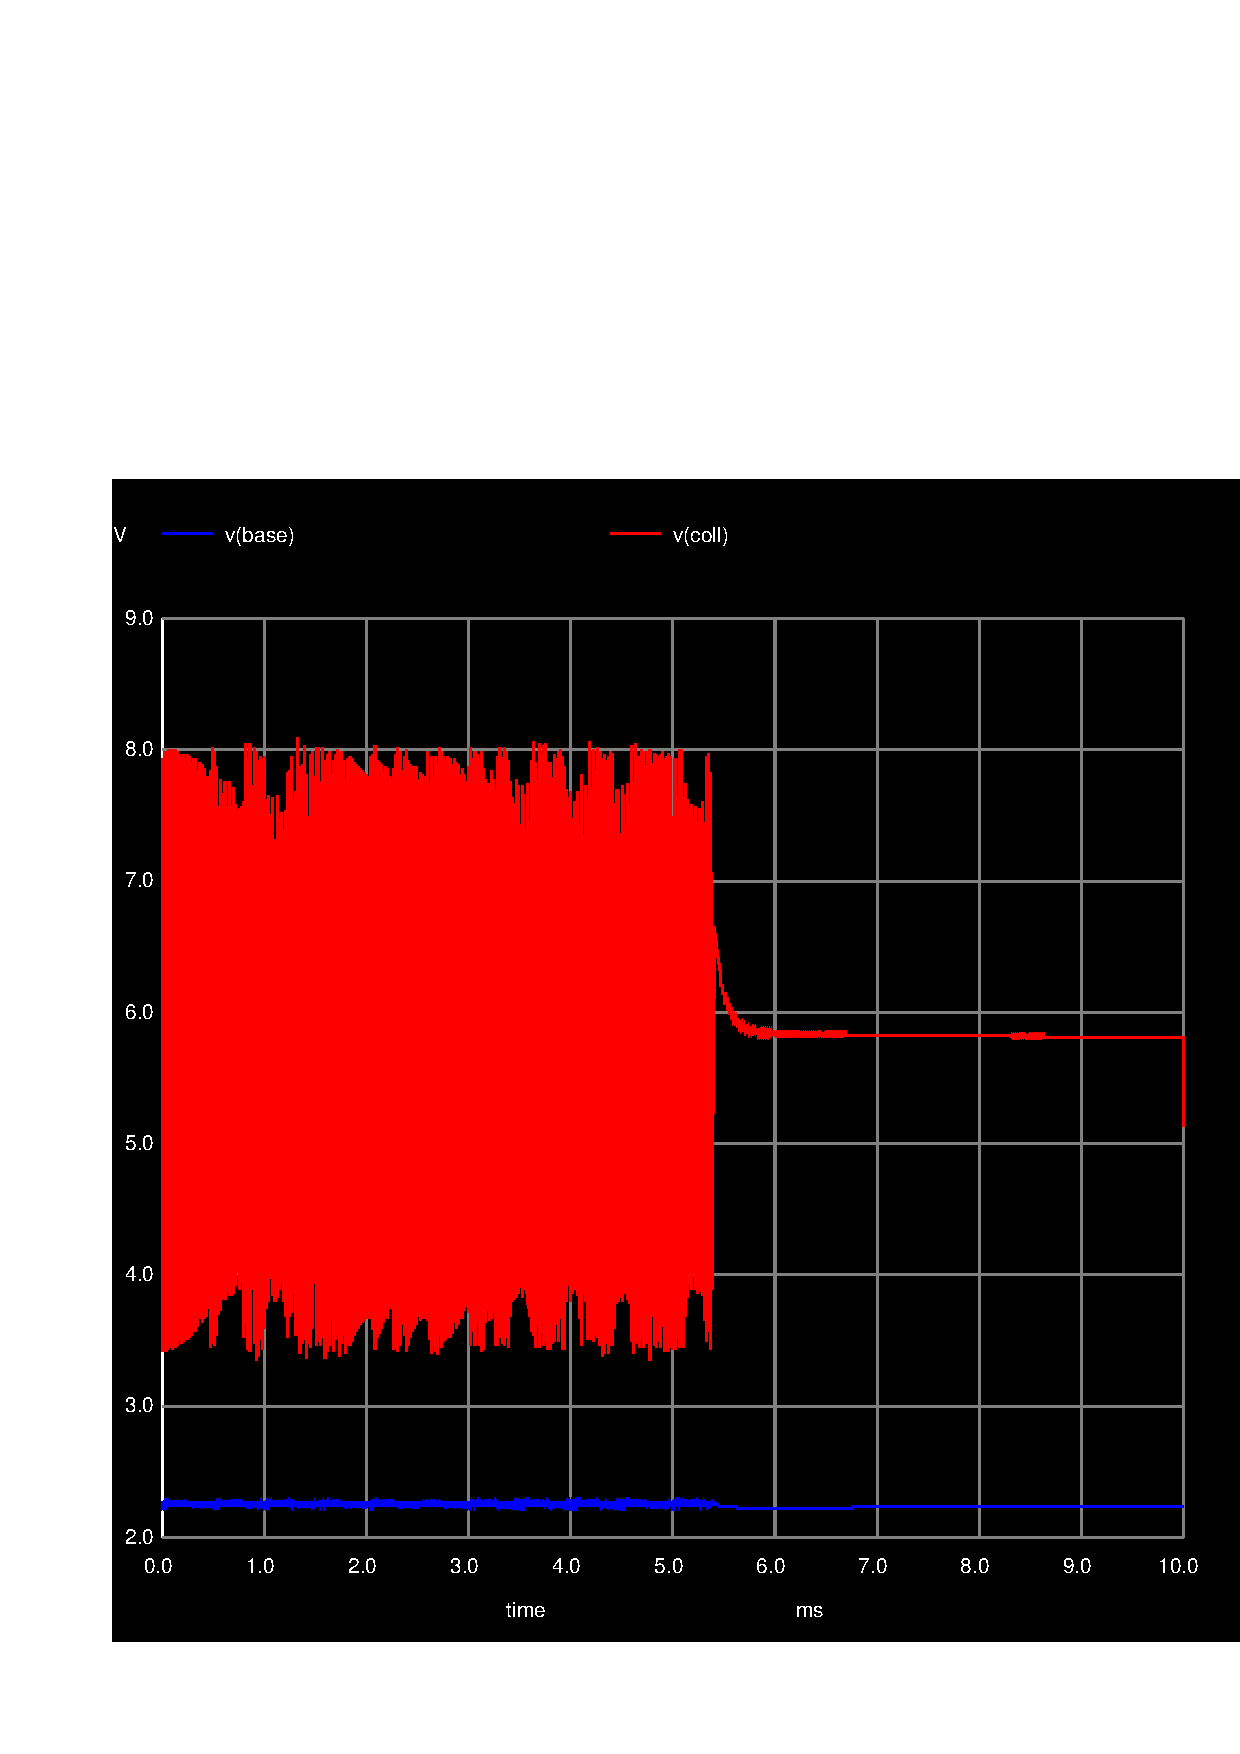
\includegraphics[width=\linewidth]{trans.pdf}
      \caption{Simulation Question 3}
    \endminipage\hfill
\end{figure}
\vspace{0.1cm}
\begin{figure}[H]
    \minipage{0.5\textwidth}
      \includegraphics[width=\linewidth]{theo5_tab.pdf}
      \caption{Theoretical Question 5}
    \endminipage\hfill
    \minipage{0.5\textwidth}
      \includegraphics[width=\linewidth]{transv5vs.pdf}
      \caption{Simulation Question 4}
    \endminipage\hfill
\end{figure}
\vspace{0.1cm}
\begin{figure}[H]
    \minipage{0.45\textwidth} 
      \includegraphics[width=\linewidth]{freq_resp_tab.pdf}
      \caption{Theoretical Question 6 - Frequency Response}
    \endminipage\hfill
    \minipage{0.45\textwidth}
      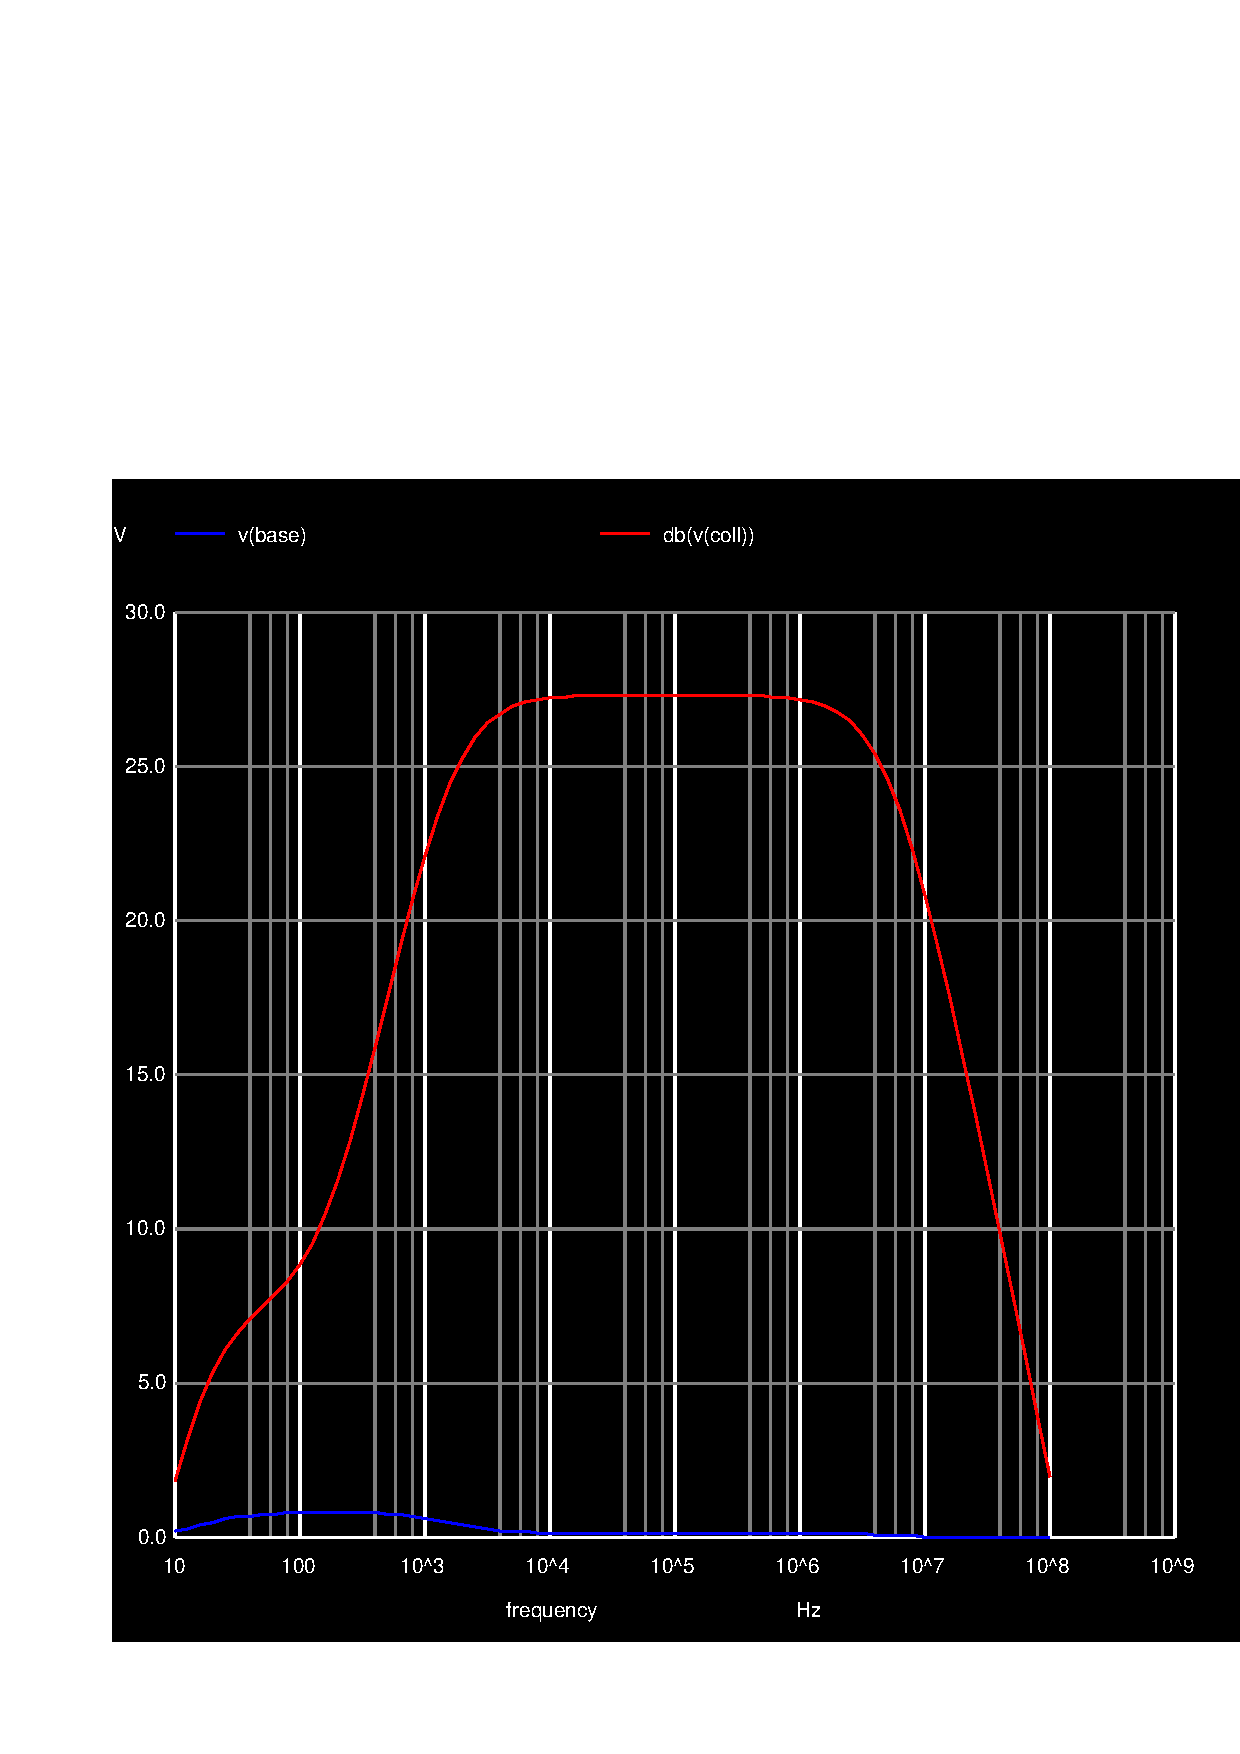
\includegraphics[width=\linewidth]{acm.pdf}
      \caption{Simulation Question 5 - Frequency Response}
    \endminipage\hfill
\end{figure}
\vspace{0.1cm}

\begin{figure}[H]
    \minipage{0.5\textwidth} 
      \includegraphics[width=\linewidth]{angle_tab.pdf}
      \caption{Theoretical Question 6 - Phase}
    \endminipage\hfill
    \minipage{0.5\textwidth}
      \includegraphics[width=\linewidth]{phase.pdf}
      \caption{Simulation Question 6 - Phase}
    \endminipage\hfill
\end{figure}
